\chapter{Аналитический раздел}

В области восстановления трехмерной формы объектов существует несколько подходов,
каждый из которых обладает своими особенностями и сферами применения.
Выбор метода зависит от требований к результату реконструкции, типа сцены, доступных данных и способов их получения.

В рамках данной работы будут рассмотрены методы восстановления глубины по единственному изображению:
\begin{itemize}
    \item структурного освещения,
    \item определения глубины из размытия (Depth from defocus)~\cite{dfd},
    \item комфортной генерации глубины (Comfortable Depth Generation),
    \item на основе нейронных сетей,
    \item восстановления глубины по закраске (Structure From Shadowing)~\cite{zaharov2011, zaharov2014}.
\end{itemize}

Задачами данного раздела являются:
\begin{itemize}
    \item обзор и сравнительный анализ существующих решений в области трехмерной реконструкции,
    \item формулировка цели работы,
    \item описание задач ВКР в виде функциональной модели.
\end{itemize}

\section{Метод структурного освещения}

В методе структурированного освещения используются различные типы световых паттернов,
которые проецируются на поверхность объекта.
Данные паттерны могут быть линейными, шахматными, градиентными и другими.
Пример паттерна представлен на изображении~\ref{pattern}.

\begin{figure}[H]
    \centering
    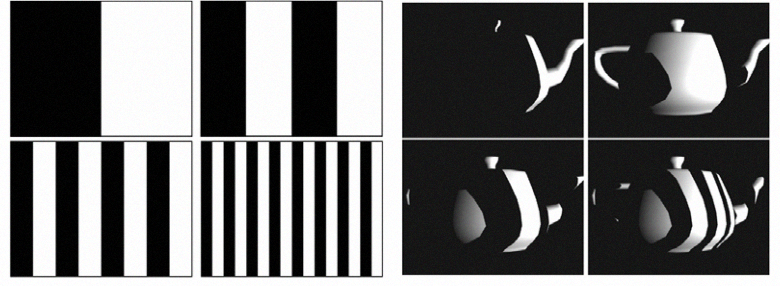
\includegraphics[scale=0.5]{img/pattern}
    \caption{Пример бинарных световых паттернов и освещенного с их помощью объекта~\cite{structLight}.}
    \label{pattern}
\end{figure}

Анализ искажений световых паттернов на поверхности объекта позволяет восстанавливать 3Д-геометрию объекта.
Основная задача метода заключается в выполнении триангуляции для определения расстояния от камеры до каждой точки поверхности.

На рисунке~\ref{metod1} приведена схема установки.

\begin{figure}[H]
    \centering
    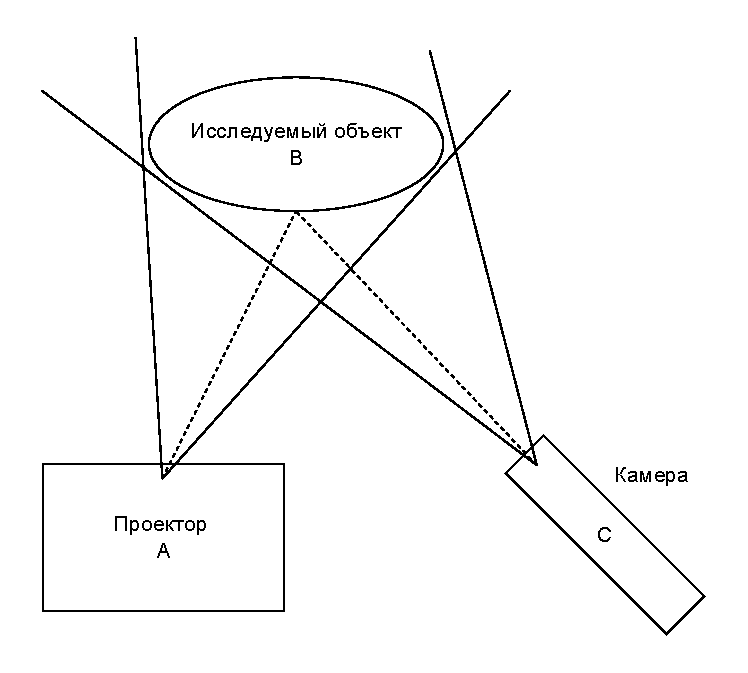
\includegraphics[scale=0.8]{img/metod1}
    \caption{Схема установки структурного освещения~\cite{structLight}.}
    \label{metod1}
\end{figure}

Создание карты глубин методом структурного освещения выполняется в несколько этапов~\cite{structLight}.

\begin{enumerate}[label=\arabic*.]
    \item \textbf{Калибровка камеры и проектора.} Определяются коэффициенты масштабирования ($\alpha_u$, $\alpha_v$), координаты оптического центра $(x_0, y_0)$ и фокусное расстояние $f$.
    \item \textbf{Проекция паттерна.} Проектор создает определенный световой шаблон (паттерн), который проецируется на исследуемую поверхность.
    \item \textbf{Фиксация изображения.} Камера фиксирует и регистрирует искажения паттерна на поверхности объекта.
    \item \textbf{Триангуляция.}
    \begin{enumerate}[label=\arabic{enumi}.\arabic*.]
        \item \textbf{ Вычисление углов.}

        Для вычисления расстояния от камеры до точки поверхности необходимо определить два угла треугольника \( \triangle ACB \):
        \begin{itemize}
            \item \( \angle CAB \) — угол между направлением от камеры \( C \) к проектору \( A \) и направлением от камеры \( C \) к точке на поверхности \( B \). Он вычисляется по формуле:
            \[
            \angle CAB = \arctan\left(\frac{x' - x_0}{f}\right),
            \]
            где \( x' \) — горизонтальная координата пикселя на изображении, \( x_0 \) — координата оптического центра камеры, а \( f \) — фокусное расстояние.

            \item \( \angle BCA \) — угол между направлением от точки \( B \) на поверхности к камере \( C \) и направлением от точки \( B \) к проектору \( A \). Он вычисляется по формуле:
            \[
            \angle BCA = \arctan\left(\frac{y' - y_0}{f}\right),
            \]
            где \( y' \) — вертикальная координата пикселя на изображении, \( y_0 \) — координата оптического центра камеры, а \( f \) — фокусное расстояние.
        \end{itemize}

        \item \textbf{Вычисление глубины $(BC)$ для каждой точки поверхности.}

        Используется триангуляция для определения расстояния \( BC \) от камеры до точки поверхности объекта:
        \begin{equation}
        BC = \frac{AC \cdot \sin(\angle CAB)}{\sin(\angle BCA)},
        \end{equation}
        где:
        \begin{itemize}
            \item \( AC \) — известное расстояние между камерой и проектором;
            \item \( \angle CAB \) и \( \angle BCA \) — углы треугольника \( \triangle ACB \), вычисляемые на предыдущем шаге.
        \end{itemize}

        \item \textbf{Преобразование координат изображения из 2Д- в 3Д-пространство.}

                Трёхмерные координаты точки поверхности \( (x, y, z) \) в системе камеры вычисляются по следующим формулам:
        \begin{equation}
        x = (x' - x_0) \cdot \frac{z}{\alpha_u}, \quad y = (y' - y_0) \cdot \frac{z}{\alpha_v}, \quad z = BC,
        \label{xyformula}
        \end{equation}
        где:
        \begin{itemize}
            \item \( x', y' \) — пиксельные координаты точки на изображении;
            \item \( \alpha_u, \alpha_v \) — коэффициенты масштабирования камеры по горизонтали и вертикали;
            \item \( x_0, y_0 \) — координаты оптического центра камеры.
        \end{itemize}
    \end{enumerate}
\end{enumerate}


Метод структурного освещения позволяет создавать точные и детализированные карты глубин,
что делает его незаменимым для решения задач,
в которых требуется высокая точность в определении расстояний до объектов.
Однако необходимым условием его использования является наличие специализированной лабораторной установки,
включающей камеру и проектор с точной калибровкой.
Такая установка требует стабильных условий и чувствительна к внешним факторам,
таким как освещенность или движение объекта.

Кроме того, метод ограничен размером и геометрией исследуемого объекта.
Структурированное освещение наиболее эффективно работает на объектах с относительно простой и ровной поверхностью.
Для сложных, сильно текстурированных или отражающих объектов,
качество получаемых данных значительно ухудшается из-за искажений паттернов,
что требует дополнительных техник для их компенсации.
Также метод неэффективен в условиях с ограниченным пространством,
где сложно разместить проектор и камеру под нужным углом.

\section{Метод определения глубины из размытия}

Метод оценки расстояний с использованием дефокусировки (Depth from Defocus, DFD) основан на анализе размытия изображения в точках, соответствующих границам объектов.
Предполагается, что перепад яркости на нерасфокусированном изображении границ объектов можно моделировать как ступенчатую функцию --- функцию Хевисайда~\cite{hewiside}.

Процесс оценки размытия выполняется в несколько этапов~\cite{dfd}.

\begin{enumerate}[label=\arabic*.]
\item \textbf{Выделение границ объектов.}
На изображении выделяются границы объектов, где наблюдаются значительные перепады яркости.
Эти границы служат ориентиром для дальнейшего анализа.
\item \textbf{Моделирование градиента яркости.}
Оценивается градиент яркости на выделенных границах объектов.
Этот шаг позволяет точно выявить изменения яркости, которые обусловлены дефокусировкой.
\item \textbf{Повторное размытие изображения.}
На изображение наносится дополнительное размытие, после чего вычисляется новый градиент яркости на границах объектов.
Это помогает уточнить степень дефокусировки, которая напрямую зависит от расстояния до объекта.
\item \textbf{Расчет параметра дефокусировки.}
На основе измерений градиента яркости и моделирования размытия вычисляется параметр дефокусировки, который используется для определения расстояния до объекта.
\end{enumerate}

Метод DFD показывает наилучшие результаты в случаях, когда есть возможность получить несколько снимков объекта с разными уровнями фокусировки.
Однако, результативность данного метода зависит от качества и точности модели размытия, а также от разрешения камеры.
В случае значительных искажений, например, при сильной дефокусировке или недостаточной контрастности на границах,
результаты менее точные.
Кроме того, для получения корректных результатов требуется тщательная настройка параметров камеры,
таких как диафрагма и фокусное расстояние.

\section{Метод комфортной генерации глубины}

Метод комфортной генерации глубины представляет собой подход,
который использует информацию о цветовых характеристиках блоков изображения для вычисления расстояния до объекта.

Процесс заключается в разбиении изображения на блоки, анализе их цветовых характеристик и применении минимальных остовных деревьев~\cite{minderev} для вычисления глубины.

Выделяют несколько основных этапов метода комфортной генерации глубины~\cite{comf}.

\begin{enumerate}[label=\arabic*.]
\item \textbf{Разбиение изображения на блоки.}
Изображение делится на блоки размером 4x4 пикселя, что позволяет упростить задачу обработки изображения и снизить вычислительную сложность.

\item \textbf{Вычисление среднего цвета для каждого блока.}
Для каждого блока вычисляется среднее значение цвета (mean(a)),
что представляет собой характеристику блока, на основе которой будет строиться граф для дальнейшей обработки.

\item \textbf{Построение графа.}
Изображение представляется как неориентированный граф \(G(V, E)\), где:
\begin{itemize}
    \item \(V\) — вершины графа, которые соответствуют блокам изображения;
    \item \(E\) — ребра графа с весами, которые рассчитываются как абсолютное различие средних значений цвета между соседними блоками, то есть \(|\text{mean(a)} - \text{mean(b)}|\).
\end{itemize}

\item \textbf{Построение минимального остовного дерева.}
На основе построенного графа применяется алгоритм Прима~\cite{prima} для нахождения минимального остовного дерева.
Этот шаг помогает упорядочить блоки по их взаимному сходству и устанавливает структуру для дальнейшего анализа.

\item \textbf{Разрезание дерева.}
После построения минимального остовного дерева выполняется его разрезание по ребрам с большими весами, что помогает выделить сегменты изображения, которые могут быть интерпретированы как части с различной глубиной.

\item \textbf{Выбор базового градиента глубины.}
Из анализа прямых линий на изображении выбирается один из базовых градиентов глубины.
Для этого используются параметры \(Wrl\) и \(Wud\), которые характеризуют градиент в двух направлениях (горизонтальном и вертикальном).
При этом выполняется условие \(|Wrl| + |Wud| = 1\).

\item \textbf{Вычисление глубины сегмента.}
Для каждого сегмента изображения глубина вычисляется как среднее значение глубины всех пикселей в сегменте.

\end{enumerate}

На рисунке~\ref{comf} приведен пример обработки одного блока изображения.

\begin{figure}[H]
    \centering
    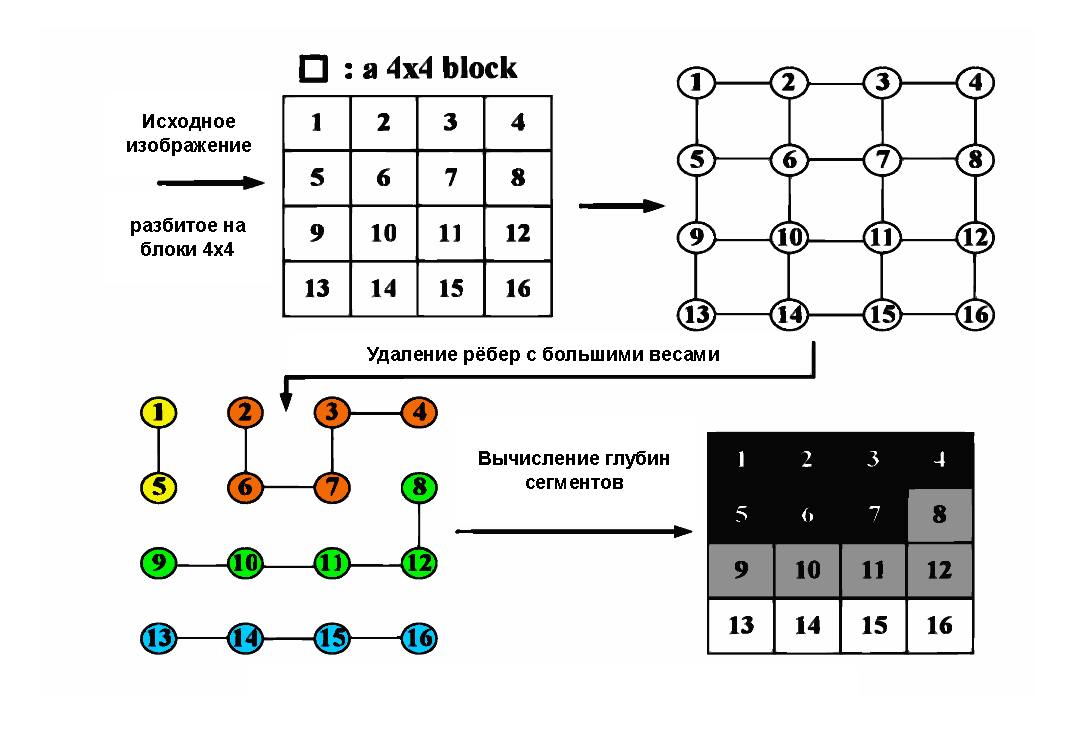
\includegraphics[scale=0.9]{img/comf}
    \caption{Обработка блока изображения~\cite{comf}.}
    \label{comf}
\end{figure}

Метод комфортной генерации глубины предполагает разбиение изображения на независимые части,
что позволяет обрабатывать данные параллельно.
Этот подход отличается универсальностью применения, поскольку может обрабатывать как локальные, так и глобальные сцены, не требуя при этом дополнительной информации или специального подхода к сбору данных.

Однако, метод Comfortable Depth Generation имеет некоторые ограничения,
связанные с качеством исходных изображений.
Низкое качество или низкая контрастность изображения снижает точность получаемой глубины.
Кроме того, фиксированный размер блоков (4x4 пикселя) ограничивает точность при обработке изображений с детализированными структурами,
требующими разделение на более мелкие части.
В случае с изображениями, содержащими гладкие или однотонные текстуры,
блоки имеют схожие цветовые характеристики,
что затрудняет выделение различных глубинных уровней.

\section{Метод восстановления глубины на основе нейронных сетей}

Методы восстановления глубины на основе нейронных сетей используют глубокое обучение для
выявления сложных статистических закономерностей между визуальными признаками 2D-изображения и соответствующими значениями глубины~\cite{shestopalov2024, istomin2024}.

Алгоритмы монокулярной оценки глубины можно разделить на несколько категорий в зависимости от их архитектуры
и подходов~\cite{istomin2024}.
Первая категория --- это предсказание глубины на основе свёрточных нейронных сетей (CNN)~\cite{istomin2024, istomin10}.
Свёрточные нейронные сети применяются для прямого предсказания карты глубин из изображения.
Обычно этот процесс заключается в обучении сети на наборах данных, содержащих пары изображений и соответствующих им карт
глубин, что позволяет модели эффективно улавливать глубинные характеристики сцены.

Второй тип архитектур --- это кодировщик-декодировщик,
в которых кодировщик отвечает за извлечение признаков из изображения, а декодировщик использует эти признаки для восстановления карты
глубин~\cite{istomin2024, istomin12}.
Такая структура позволяет более эффективно моделировать сложные зависимости в изображениях, что
повышает точность результата~\cite{istomin2024}.

Одним из представителей нейросетевых методов является модель MiDaS,
предназначенная для оценки глубины на основе одиночных изображений, которая характеризуется гибридной архитектурой,
объединяющей элементы кодера-декодера в рамках свёрточной нейронной сети~\cite{istomin2024, istomin12}.

MiDaS обучен на комбинированных наборах данных, что обеспечивает его универсальность для разных типов сцен
и устойчивость к шумам и артефактам.
Кроме того, важным преимуществом является отсутствие необходимости в знании точных параметров камеры и какой-либо дополнительной информации.
Однако, как и метод Comfortable Depth Generation, нейросетевые подходы ориентированы на восстановление общей структуры глубины, упуская детали поверхностей.

\section{Метод восстановления глубины по закраске изображения}

Метод Shape from Shading (SFS) --- это подход к восстановлению трехмерной формы объекта на основе анализа распределения интенсивности света и теней на двумерном изображении.
Этот метод базируется на физических принципах отражения света от поверхностей объектов.

Восстановление формы по закраске производится в несколько этапов~\cite{stanowski2024stability}.

\begin{enumerate}[label=\arabic*.]
\item \textbf{Определение модели освещения.}
Для анализа используется модель отражения, описывающая взаимосвязь между интенсивностью пикселя, нормалью к поверхности и направлением падающего света. Чаще всего применяется ламбертовская модель освещения:
\begin{equation}
I(x,y) = \rho(x,y) \cdot L \cdot N(x,y),
\end{equation}
где $I(x,y)$ --- интенсивность пикселя, $\rho(x,y)$ --- альбедо поверхности, $L$ --- направление источника света, $N(x,y)$ --- нормаль к поверхности.

\item \textbf{Разделение альбедо и затенения.}
Анализируется изменение яркости изображения для отделения свойств материала (альбедо) от эффектов затенения, вызванных геометрией поверхности.
Альбедо характеризует собственный цвет и отражательную способность материала.

\item \textbf{Вычисление нормалей поверхности.}
На основе интенсивности пикселей и модели освещения вычисляются нормали к поверхности в каждой точке.
Для каждого пикселя определяется вектор нормали $N(x,y)$, перпендикулярный к касательной плоскости поверхности.

\item \textbf{Интеграция нормалей.}
Для получения карты глубин выполняется интеграция поля нормалей.
Этот процесс можно представить как решение следующего уравнения:
\begin{equation}
\nabla Z(x,y) = f(N(x,y)),
\end{equation}
где $Z(x,y)$ --- искомая карта глубины, а $f$ --- функция, преобразующая нормали в градиент глубины.

\item \textbf{Применение регуляризации.}
Для преодоления неоднозначности решения и устранения шумов используются методы регуляризации, которые вводят дополнительные ограничения на гладкость поверхности.
\end{enumerate}

Метод SFS обладает рядом преимуществ, ключевым из которых является возможность восстановления 3D-формы объекта по одиночному изображению.
Это делает его применимым для работы с историческими фотографиями, когда невозможно получить несколько ракурсов объекта~\cite{xie2025photometric}.

Однако метод имеет существенные ограничения.
Во-первых, он требует точного знания параметров освещения, которые часто недоступны для архивных фотографий.
Во-вторых, базовая модель предполагает однородность материала поверхности, что редко встречается в реальных сценах.
В-третьих, метод дает неоднозначные результаты, поскольку различные 3D-формы могут создавать схожие паттерны затенения~\cite{zhang2025review}.


